  %%%%%%%%%%%%%%%%%%%%%%%%%%%%%%%%%%%%%%% -*- coding: utf-8; mode: latex -*- %%
  %
%%%%%                         CHAPTER
 %%%
  %

% $Id: 1020-lorem-ipsum.tex,v 1.2 2009/06/19 15:51:46 david Exp $
% $Log: 1020-lorem-ipsum.tex,v $
% Revision 1.2  2009/06/19 15:51:46  david
% *** empty log message ***
%
% Revision 1.1  2007/11/23 09:52:39  david
% *** empty log message ***
%
%

  %%%%%%%%%%%%%%%%%%%%%%%%%%%%%%%%%%%%%%%%%%%%%%%%%%%%%%%%%%%%%%%%%%%%%%%%%%%%%
  %
%%%%%                           HEAD MATTER
 %%%
  %

\chapter{Background and Related Work}
%\addcontentsline{lof}{chapter}{\thechapter\quad Lorem Ipsum}
%\addcontentsline{lot}{chapter}{\thechapter\quad Lorem Ipsum}
\label{ch:bkgAndRw}

\section{Hadoop File System(HDFS)}
Apache Hadoop ~\cite{h17} is an open-source software framework for large-scale data
processing. It includes a distributed file system called the Hadoop Distributed
File System (HDFS) and a framework for MapReduce. Many data analysis,
data warehousing and machine learning solutions have been built on top of it.
The most commonly known extensions of Hadoop are Apache Pig ~\cite{21}, Apache
Hive ~\cite{22}, Apache HBase  ~\cite{26}, Apache Zookeeper  ~\cite{27} and Apache Mahout  ~\cite{23}.
Recent version of Hadoop also include a resource negotiator called Yet-Another-
Resource-Negotiator (YARN), often also referred to as NextGen MapReduce or
short MRv2. YARN is, inter alia, used to execute MapReduce jobs. The design
and concepts used by Hadoop are inspired by the Google papers about GFS and
MapReduce ~\cite[p.~9]{h17}. Similar to MapReduce on GFS, Hadoop is exploiting data
locality for MapReduce jobs by trying to execute map jobs on a DataNode which
hosts the data. If not possible, the framework will attempt to execute the job
on a node close to the location of data, for instance on the same rack. This can
greatly improve the overall performance  and reduces the network bandwidth
requirements.\\
 HDFS  is   Hadoop’s   distributed  file  system   which  has   been  designed  after  Google  File System.It was initially created to be used in a Map-Reduce computational framework of Hadoop by Apache though later on it started to be used for other big data applications as a storage which can support massive amount of data on commodity machines. Hadoop File System were intended to be distributed for being accessed and used inside by distributed processing machines of Hadoop with a short response time and maximum parallel streaming factor. On the other hand, in order for HDFS to be used as a storage of immutable data for applications like Facebook, the high availability is a key requirement besides the throughput and response time. Moreover, as a file system to be compliant to the common file system standard, it provides posix like interface in terms of operations, however it has a weaker consistency model than posix which is being discussed later on in this section.
 \subsection{HDFS Architecture}
HDFS  splits   up  each  file  into  smaller  blocks  and replicates  each block  on a different random
machine.  Machines   storing  replicas   of  the  blocks   called  DataNode. On the other hand since
it  needs   to  have  namespace  metadata  accessible  altogether,  there  is   a  dedicated metadata
machine  called  NameNode.  For  having  fast  access   to  metadata,  NameNode  stores
metadata  in  memory.  Accessing  to  HDFS  happens   through  its   clients,  each  client  asks
NameNode  about  namespace  information,  or  location  of  blocks   to  be  read  or  written, then it
connects   to  DataNodes   for  reading  or  writing  file  data.  Figure\ref{fig:HDFS_Architecture}  shows   the  deployment  of
different nodes in HDFS.
\begin{figure}[htb]
  \centering
 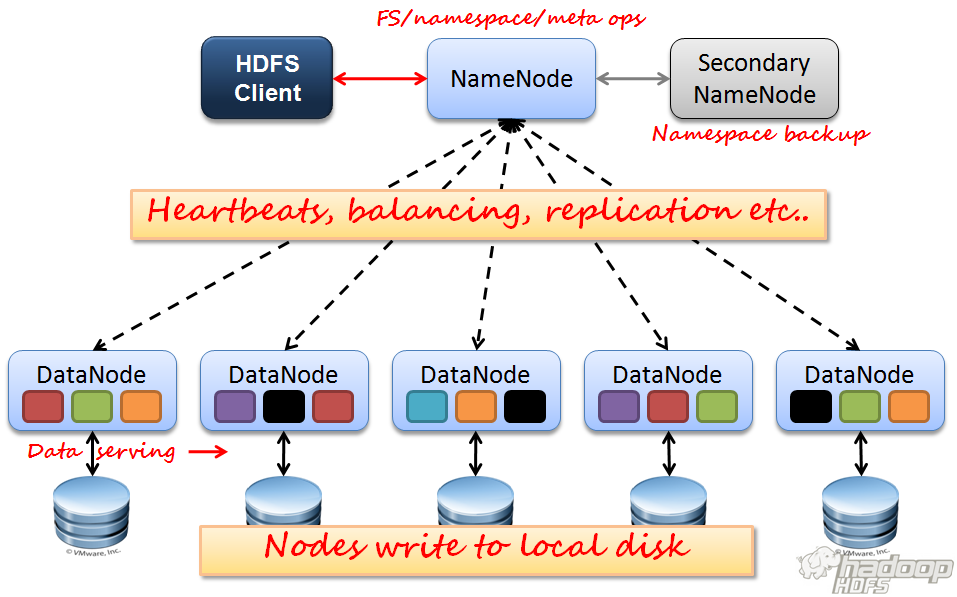
\includegraphics[scale=0.5]{figs/preliminar/HDFS_Architecture.png}
  \caption{HDFS Architecture.}
  \label{fig:HDFS_Architecture}
\end{figure}
\subsection{HDFS NameNode}
NameNode  is   known  as   metadata  server  of  HDFS. Its  multithreaded server in which size of
the  thread  pool  is   configurable.  It  keeps   all  metadata  information  in  memory   which  is
described  in  the  next  section.  The  way   NameNode  protects   race  condition  for  metadata
modification  is   based  on  read/write  lock.  It  splits   all  operations   into  read  or  write  operations.Its procedure is shown in alogithm \ref{NormalNameNode}.In this way multiple read operations could be run in parallel though they are serialized with
each single write operation.
Other  than  serving  client’s   requests,  NameNode  has   been  serving  part  for  DataNodes,  via
this   service. DataNodes  notice NameNode about receiving or deletion of blocks  or they  send
over  list  of  their  replicas   periodically.  Moreover,  NameNode  has   one  still running  thread
namely   ReplicationMonitor  to  get  under-replication  and  over-replication  under  its   radar  and
plans for deletion/replication accordingly.
Moreover,  LeaseMonitor  controls   the  time  limit  that  each  client  holds   the  write  operation  of files.  So  it  walks   through  all  leases   and  inspect  their  soft-limit/hard-limit  and  decides   to
recover or revoke an expired lease.

\begin{algorithm}[h]
\caption{System-Level locking schema in HDFS}
\label{NormalNameNode}
\begin{algorithmic}
\State \textbf{Operation } lock
\If { op.type = write }
\State ns.acquireWriteLock()
\Else
\State ns.acquireReadLock()
\EndIf\\
\State \textbf{Operation }  perform Task
 \State //Operation body \\
\State \textbf{Operation } unlock
\If { op.type = write }
\State ns.releaseWriteLock()
\Else
\State ns.releaseReadLock()
\EndIf
 

\end{algorithmic}
\end{algorithm}

\subsection{HDFS consistency model}
\begin{enumerate}
\item \textbf{FileSystem Operations}\\
In  general  most  of  the  distributed  file  systems   like  GFS  and  HDFS  have  a  relaxed
version  of  consistency   because  of  the  impossibility   result  of  CAP  theorem \cite{cap}
which  limits   scalability   of  file  system.  Even  though  some  works   refer  to  HDFS  as
sequential  consistent  file  system   for  data  and  from   filesystem   operations   point  of
view,  it  does   not  certainly   have  sequential  consistency   due  to  nonatomic   write
operation.  HDFS  serializes   read/write  operations  just at the primitive operations’ level
not  the  files   blockdata.  As  each write operations  consists  of multiple micro addBlock
operations   which  makes   it  unsortable  when  multiple  parallel  reads   are  being
performed with one write. Though it protects  multiple writes  by  means  of a persistable
mechanism called lease.
\item \textbf{Primitive NameNode Operations}\\
From   primitive  operations   point  of  view, HDFS is  strongly  consistent in both data and
metadata level.
From   data  level  it  is   strongly   consistent  because  each  file’s   block   is  not available for
read  unless   it  gets   completely   replicated.  It  means   write  operation  should  be
completely   finished  first,  then  readers   will  all  get  the  same  version  of  that  block   and
there is not case of version mismatch in the replicas read by two different readers.
From   metadata  level,  as   already   been  mentioned, system  level lock  serializes  all the
write  operations   which  results   in  mutated  state  of  all  writes   bing  available  for  all
readers.

\end{enumerate}

\subsection{POSIX compliant filesystem}
POSIXfs   is   file  system   part  of  POSIX  operating  system.  It  has   been  being  a  standard  for
designing  filesystems.  It  is   about  naming,  hardlinks,  access   control,  time  stamping  and
standard  folder  hierarchy.  Under  POSIX  standards,  almost  all  file  operations   shall  be
linearized.  Specifically   all  read  operations   should  have  effects   of  all  previous   write
operations.
HDFS  is   not  fully  POSIX compliant, because the requirements  for a POSIX file system  differ
from   the  target  goals   for  a  Hadoop  application.  The  tradeoff  of  not  having  a  fully
POSIXcompliant  file  system   is   increased  performance  for  data  throughput  and  support  for
nonPOSIX  operations   such  as   Append.  Moreover,  HDFS  consistency   model  is   weaker
than  POSIX.  HDFS  is   strongly   consistent  from   primitive  HDFS  operations   while  from
filesystem   operations   it  has   a  relaxed  version  of  consistency,  on  the  other  hand,  POSIX
filesystem operations are linearizable which is the highest level of consistency.

\section{Hadoop Open Platform as Service(HOP)-HDFS}

Hadoop Open Platform as a service (HOP) \cite{10} is a Hadoop distribution based
on Apache Hadoop . It provides namespace scalability through the support of multiple
NameNodes, platform as a service support for creating and managing clusters,
and a dashboard for simplified administration. HOP is developed in cooperation
of KTH and SICS \cite{15}\\
HOP-HDFS\cite{11} \cite{12} is a fork of HDFS and part of HOP. It aims on providing high
availability and scalability for HDFS. This is achieved by making the NameNode
stateless and thereby adding support for the use of multiple NameNodes at the
same time. Instead of storing any state in the NameNode, the state is stored in
a distributed database offering high-availability and high-redundancy. Therefore,
the current implementation uses MySQL Cluster \cite{29}, which utilizes NDB Cluster
as an underlying storage engine.
HOP-HDFS is a promising approach that could make HDFS similar to Colos-sus, while overcoming the scalability and availability limitations of the current
Hadoop implementation. Through its support for larger amounts of metadata, it
could also make the use of block sizes smaller than 64 megabytes efficient, what
might be useful for many applications.



  %%%%%%%%%%%%%%%%%%%%%%%%%%%%%%%%%%%%%%%%%%%%%%%%%%%%%%%%%%%%%%%%%%%%%%%%%%%%%
  %
%%%%%                         ANOTHER SECTION
 %%%
  %
\subsection{HOP-HDFS Architecture}
The persistent data structures of HOP-HDFS (here after referred as HDFS) are defined as 11 database tables. These tables contain all the information about namespace,metadata,block locations and many other information that name-node in HDFS stores in FSImage and keeps in memory.
\begin{enumerate}
\item \textbf{inodes:} The  table  representing  inode  data  structure  in  HDFS  which  contains   the namespace  and  metadata  of  the  files   and  directories.  inodes   are  related  together  by their  parent\_ id  and  resembles   a  hierarchical  namespace  as   in  the  HDFS.  Each  row has a unique id which is the primary key.
\item \textbf{block\_ inofs:} Block   is   a  primitive  of  HDFS  storing  a  chunk   of  a  file,  block-info  is   its
metadata  keeping  a  reference  to  its   file-inode,  the  list  of  block’s   replica  which  are
scattered among multiple data-nodes.
\item \textbf{leases:} Basically   each  file  in  HDFS  is   either  underconstruction  or  completed.  All
underconstruction  files   are  assigned  a  sort  of  write  lock   to  them,  this   lock   is
persisted  in database. Each lease corresponds  to just one client machine, each client
could be writing multiple files at a time.

\item \textbf{lease\_ path:} Each  lease  path  represents   an  underconstruction  file, it holds  full path
of that file and points to the lease as its holder.

\item \textbf{replicas:} A  copy   of  a  Block   which  is   persisted  in  one  datanode,  sometime we refer
to replicas as blocks. All the replicas of the same block points to the same blockinfo.

\item \textbf{corrupted\_ replicas: }A replica become corrupted in the copy  operations  or due to the
storage  damages.  Namenode  realizes   this   by   comparing  checksum   in  the  report of
the replica’s datanode with the checksum of the original block.

\item \textbf{excess\_ replicas:} A  block   could  become  over replicated because of an already  dead
datanode  coming  alive  again  and  contain  some  replicas   which  has   been  removed
meanwhile  from   namenode.  So  distinguishing  that,  namenode  marks   marks   some
replicas to be removed later on.

\item \textbf{invalidated\_ blocks:} For  every   datanode  keeps   a  list  of  blocks   that  are  going  to  be
invalidated(removed) on that datanode due to any reason.

\item \textbf{replicas\_ under\_ construction:} Replications   of  a  block   which  are  being  streamed  by
client into datanodes.

\item \textbf{under\_ replicated\_ blocks:} Keeps   track   of  the  blocks   which  has   been  under
replicated,  it  realizes   the  priority   of  under  replications   as   follow.  Priority   0  is   the
highest  priority.  Blocks   having  only   one  replica  or  having  only   decommissioned
replicas   are  assigned  priority   0.  Blocks   having  expected  number  of  replicas   but  not
enough  racks   are  assigned  with  priority   3.  If  the  number  of  replicas   of  a  block   are  3
times   less   than  expected  number  of  replicas   then  the  priority   is   assigned  to  1.  The
rest  of  low  replication  cases   are  assigned  priority   2.  Blocks   having  zero  number  of
replicas   but  also  zero  number  of  decommissioned replicas  are assigned priority  4 as
corrupted blocks.

\item \textbf{pending\_ blocks:} Represents a blocks that are being replicated.

\end{enumerate}
 The figure \ref{fig:HDFS_table_relation} illustrates the relation between tables. The figure \ref{fig:HDFS_table_schema} gives the columns stored in each table.
\begin{figure*}
  \centering
 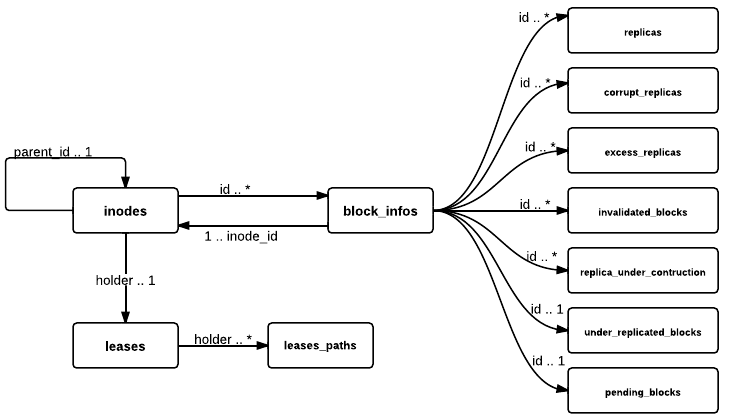
\includegraphics[scale=0.5]{figs/preliminar/HOP_table_relation.png}
  \caption{HOP-HDFS Table relations.}
  \label{fig:HDFS_table_relation}
\end{figure*}
\pagebreak
\begin{figure*}
  \centering
 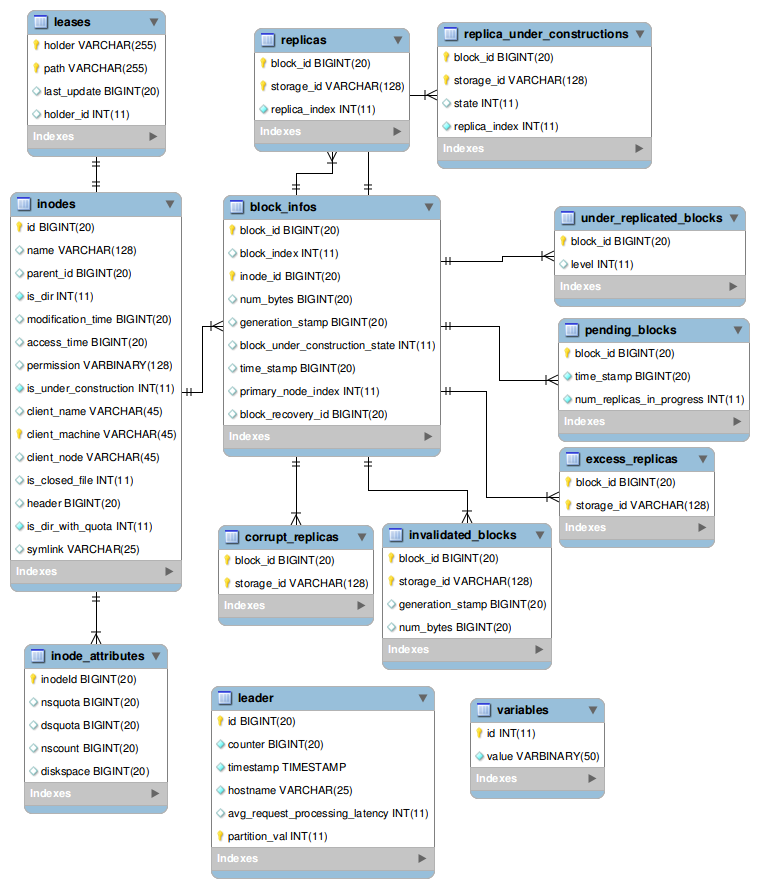
\includegraphics[scale=0.5]{figs/preliminar/HOP_HDFS_Schema.png}
  \caption{HOP-HDFS Schema}
  \label{fig:HDFS_table_schema}
\end{figure*}



  %%%%%%%%%%%%%%%%%%%%%%%%%%%%%%%%%%%%%%%%%%%%%%%%%%%%%%%%%%%%%%%%%%%%%%%%%%%%%
  %
%%%%%                          LAST SECTION
 %%%
  %

\subsection{NameNode Operations}

Every   operation  defined  in  the  HDFS  client  API  (such  as   createFile,  open,  etc)  maps   onto  one  or  more  of  the  following  primitive  HDFS  operations.  Each  operation  defined  in  the primitive  HDFS  API  maps  onto a protocol message (where each protocol message contains request, reply, and exception  parts) sent between the NameNode, client, and DataNodes. Some  common   primitive  operations  are  shown   in   the  table \ref{NameNode_Ops}.  The  full  list  of  the primitive operations can be found in Thesis report \cite{12} Appendix section.
\begin{table}[t]
\centering
\begin{tabular}{|l|p{12cm}|}
\hline
\textbf{OPERATION} & \textbf{SUMMARY}\\
\hline
\textbf{MKDIR}&Creates   a  directory   recursively,  it  requires   a  no
lock   on  all  the  existing  components   of  the  path
but  write  lock   on  the  last existing.\\
\hline
\textbf{START\_ FILE} & \begin{enumerate}
\item If  file  does   not  exist,  It  creates   inodes
for  all  the  nonexistent  directories   and
new  file,  writes   owner  of  the  lease  and
creates new leasepath.
\item If  file  already   exists   first  removes   the
file,  its   blocks   and  dependencies,  lease
and  lease  path,  then  it  does   the  first
scenario.
\end{enumerate}\\
\hline
\textbf{GET\_ ADDITIONAL\_ BLOCK}&  In  the  middle  of  writing  a  file,  this   is   the  client’s
           mean  of  noticing  namenode  that  the  already
                 being  written  block   is   finished  while  it  is   asking
                        for  the  locations   of  next  block.  NameNode
                             removes   all  the  replicaunderconstructions   of
                                  last  block, it also changes  type of blockinfo from
                                          underconstruction  to  completed  one.\\

\hline
\textbf{COMPLETE}& Like  get\_ additional\_ block,  it  happens   for  last
    block   of  the  file,  NameNode  just  removes   the
          replicaunderconstructions   and  changes   type  of
               blockinfo from underconstruction to completed.
 \\
\hline
\textbf{GET\_ BLOCK\_ LOCATIONS}& Given  path  of  the  file,  it  returns   location  if  its
        blocks and updates accesstime of the fileinode.
 \\ 
 \hline
 \textbf{DELETE} & Delete the given file or directory from the file system.\\
 \hline
 \textbf{RENAME} & Renames gives SRC to DST. Without OVERWRITE option, rename fails if the dst already exists. With OVERWRITE option, rename overwrites the dst, if it is a file 
    or an empty directory. Rename fails if dst is a non-empty directory. The rename opeartion is atomic.\\
\hline 
 \textbf{APPEND} & Append to the end of the file.It retuns the partially completed last block if any. \\
 \hline
\end{tabular}
\caption{NameNode's Operations}
\label{NameNode_Ops}
\end{table}

\subsection{HOP-HDFS Implementation}
In HOP-HDFS each HDFS opeartion is implemented as a single transaction,where after transaction began, read and write the necessary meta-data from NDB , and then either commit the transaction, or in case of failure, the transaction was aborted and then possibly retried. However,  the  default  isolation  level  of  NDB  is   read  committed,  which  allows   the  results   of
write  operations   in  transactions   to  be  exposed  to  read  operations   in  different  concurrent
transactions.  This   means   that  a  relatively   long  running  read  transaction  could  read  two
different  versions   of  data  within  the  same  transaction,  known  as  a fuzzy  read, or it could get
different  sets   of  results   if the same query  is  issued twice within the same transaction  this  is
known as a phantom read. In report\cite{12} and paper \cite{hoppaper} they proposed and implemented the snapshot-isolation method \ref{hopAlgo} which pessimistically locks the rows of data preventing other transactions from accessing. 
Transactions that contain both a read and a modify filesystem operation for the same shared metadata object should be serialized based on the serialization rule:\\\\
$ -\forall(w_{i},w_{j}) \hspace{1em} if \hspace{1em} X_{wi}\cap X_{wj} \neq \phi$ then transactions of $ (w_{i},w_{j})$ must be serialized; $
-\forall(r_{i},w_{j})  \hspace{1em} if \hspace{1em} X_{ri}\cap X_{wj} \neq \phi$ then transactions of $(r_{i},w_{j})$  must be serialized.\\\\
First, the hierarchy of the file system to define a partial ordering over
inodes. Transactions follow this partial ordering when taking locks, ensuring
that the circular wait condition for deadlock never holds. Similarly, the partial
ordering ensures that if a transaction takes an exclusive lock on a directory inode,
subsequent transactions will be prevented from accessing the directory's subtree
until the lock on the directory's lock is released. Implicit locks are required for
operations such as creating files, where concurrent metadata operations could
return success even though only one of actually succeeded. For operations such
as deleting a directory, explicit locks on all child nodes are required.

\begin{algorithm}[h]
\caption{Snapshotting taking locks in a total order}
\label{hopAlgo}
\begin{algorithmic}

\State snapshot.clear \\ \\

\textbf{Operation } doOperation \\

\State tx.begin
\State create-snapshot()
\State performTask()
\State tx.commit\\

\State \textbf{Operation} create-snapshot \\
\State S = total\_ order\_ sort(op.X) 
\ForAll{x in S}
\If{x is a parent }
\State level = x.parent\_ level\_ lock
\Else
\State level = x.strongest\_ lock\_ type
\State tx.lockLevel(level)
\State snapshot $<$- tx.find(x.query)
\EndIf
\EndFor
 \\ 
\State \textbf{Operation} performTask
\State //Operation Body,referring to transaction cache for data

\end{algorithmic}
\end{algorithm}

\section{MySQL Cluster}
Mysql  Cluster  is   a  Database  Management  System   (DBMS)  that  integrates   the  standard
Mysql  Server with an inmemory  clustered storage engine called NDB Cluster (which stands
for  “Network   DataBase”)  .  It  provides   a  sharednothing  system   with  no  single
point of failure.



Mysql  Cluster  is   a  compound  of  different  processes   called  \textbf{nodes}.  The  main  nodes   are
Mysql  Servers   (mysqld,  for  accessing  NDB  data),  data  nodes   (ndbd,  as   the  data  storage),
one  or  more  management  servers   (ndb\_ mgmd).  The  relationship  between  these  nodes   are
shown in figure \ref{fig:mysqlCluster}.
The  data  in Mysql Cluster is  replicated over multiple ndbds  so this  makes  the database to be
available  in  case  of  node  failures.  Ndbds   are  divided  into \textbf{node groups}.  Each  unit  of  data
stored  by   ndbd  is   called  a  \textbf{partition}.  The  partitions   of  data  are  replicated  into  ndbds   of  the
same node group while node groups are calculated indirectly as following:
$$Number of Node groups  = \frac{number of  datanodes}{number of  replicas} $$
A  simple  cluster  of  4  datanodes   with  replication  factor  of  2  and  consequently  2 node groups
are shown in figure \ref{fig:nodegroups}.
As   it  can  be  seen,  the  data stored in the database are divided into 4 partitions. There are two
replicas   of  each  partition  into  ndbds   of  the  same  node  group.  So  even  if  one  of the ndbds  in
each  of  the  node  groups   are  failed, the whole data in the cluster will be available. However, if
both  ndbs   in a node group become unavailable then those partitions  stored by  the failed ndbs
also will become unavailable.
According  to  a  white  paper  published  by   Oracle  ,  Mysql  Cluster  can  handle  4.3
billion  fully   consistent  reads   and  1.2  fully  transactional writes  per minute. They  used an open
source  benchmark   called  flexAsynch  and  a  Mysql  Cluster  of  30  data  nodes,  comprised  15
node  groups.  The  detail  of  their  system   configuration  is   available  in  the  referenced  white
paper. The results for write operations are shown in figure \ref{fig:mysqlCluster}.
The  72  million  reads   and  19.5  million  write  operations   per  second  of  Mysql  Cluster  shows
that it has a high throughput for simple read and write operations.
\pagebreak
\begin{figure*}
\centering  
 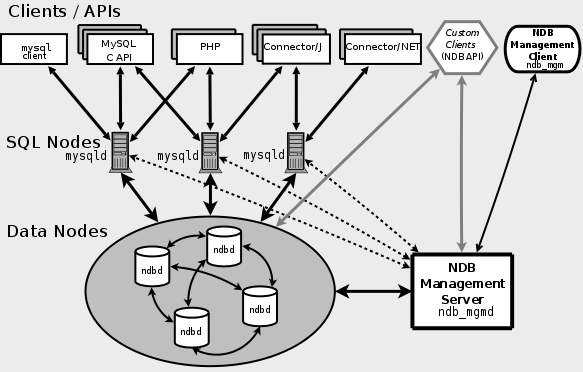
\includegraphics[scale=0.65]{figs/preliminar/mysql_cluster.png}
  \caption{MySQL cluster}
  \label{fig:mysqlCluster}
\end{figure*}

\begin{figure*}
\centering  
 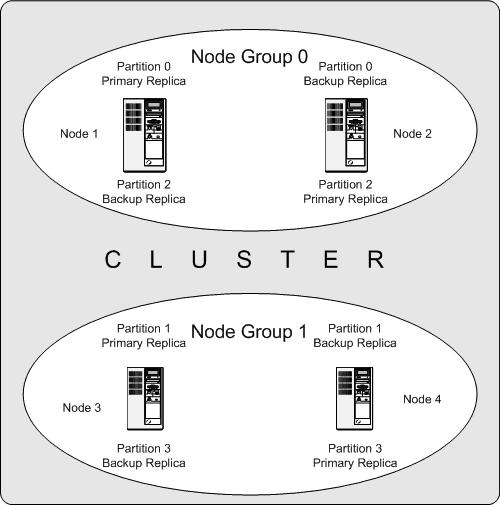
\includegraphics[scale=0.4]{figs/preliminar/nodegroups.png}
  \caption{Node groups of MySQL cluster}
  \label{fig:nodegroups}
\end{figure*}

\subsection{Concurrency Control in NDBCluster}
NDB  supports   pessimistic   concurrency   control  based  on  locking.  It  supports   row  level
locking.  NDB  throws   a timeout error if a requested lock  cannot be acquired within a specified
time \cite{mysql1}.  Concurrent  transactions,  requested  by   parallel  threads   or  applications,
reaching  the  same  row  could  end  up  with  deadlock.  So,  it  is   up  to  applications   to  handle
deadlocks   gracefully.  This   means   that  the  timed  out  transaction  should  be  rolled  back   and
restarted.  Transactions   in  NDB  are  expected  to  complete  within  a  short  period  of  time,  by
default  2  seconds.  This   enables   NDB  to  support  realtime  services,  that  are,  operations
expected  to  complete  in  bounded  time.  As   such,  NDB  enables   the  construction  of  services
that  can  failover,  on  node  failures,  within  a  few  seconds     ongoing transactions  on the node
that  dies  timeout within a couple of seconds, and its  transactions  can be restarted on another
node in the system.

\subsection{ClusterJ}
Clusterj  is   Java  connector  implementation  of  NDB  Cluster,  Mysql  Cluster’s   storage  engine, \cite{29}.  Clusterj  uses   a  JNI  bridge  to  the  NDB  API  to  have  a  direct  access   to  NDB
Cluster.  The  NDB  API  is   an  application  programming  interface  for  Mysql  Cluster  that
implements   indexes,  scans,  transactions   and  event  handling.  Clusterj  connects   directly   to
NDB  Clusters   instead  of  connecting  to  mysqld.  It  is   a  persistence  framework   in  the  style of
Java  Persistence  API.  It  provides   a  data  mapper  mapping  java  classes   to  database  tables
which separates the data from business logic.

\section{Related Work}
\subsection{Snapshots in Apache Hadoop Version2}
Apache Hadoop implemented snapshots in their latest version \cite{Hadoop2} , which supports nested snapshots and constant time for the creation of snapshots. Since metadata and data are separated it supports strong consistency for metadata snapshot but not for data.In case of file being written, unless the datanode notifies the namenode or client notifies namenode of latest length of last block via hsync, namenode is unaware of current length of the file when snapshot was being taken.The solution also couldn't address the case of replication change of half-filled last block after taking snapshot, where it is appended after taking snapshot.\\
Apache Hadoop distribution provides single snapshot mechanism to protected file system meta-data and storage-data from software upgrades. The snapshot mechanism lets administrators persistently save the current state of the filesystem, so that if the upgrade results in data loss or corruption it is possible to rollback the upgrade and return HDFS to the namespace and storage state as they were at the time of the snapshot.

The snapshot (only one can exist) is created at the cluster administrator's option whenever the system is started. If a snapshot is requested, the NameNode first reads the checkpoint and journal files and merges them in memory. Then it writes the new checkpoint and the empty journal to a new location, so that the old checkpoint and journal remain unchanged.

During handshake the NameNode instructs DataNodes whether to create a local snapshot. The local snapshot on the DataNode cannot be created by replicating the directories containing the data files as this would require doubling the storage capacity of every DataNode on the cluster. Instead each DataNode creates a copy of the storage directory and hard links existing block files into it. When the DataNode removes a block it removes only the hard link, and block modifications during appends use the copy-on-write technique. Thus old block replicas remain untouched in their old directories.

The cluster administrator can choose to roll back HDFS to the snapshot state when restarting the system. The NameNode recovers the checkpoint saved when the snapshot was created. DataNodes restore the previously renamed directories and initiate a background process to delete block replicas created after the snapshot was made. Having chosen to roll back, there is no provision to roll forward. The cluster administrator can recover the storage occupied by the snapshot by commanding the system to abandon the snapshot; for snapshots created during upgrade, this finalizes the software upgrade.

System evolution may lead to a change in the format of the NameNode's checkpoint and journal files, or in the data representation of block replica files on DataNodes. The layout version identifies the data representation formats, and is persistently stored in the NameNode's and the DataNodes' storage directories. During startup each node compares the layout version of the current software with the version stored in its storage directories and automatically converts data from older formats to the newer ones. The conversion requires the mandatory creation of a snapshot when the system restarts with the new software layout version.

\subsection{Snapshots in Hadoop at Facebook}
Facebook has implemented a solution to Snapshots \cite{Facebook}. The solution scales linearly with the number of inodes(file or directories) in the filesystem.It uses a selective copy-on-append scheme that minimizes the number of copy-on-write operations. This optimization is made possible by taking advantage of the restricted interface exposed by HDFS, which limits the write operations to appends and truncates only.The solution has space overhead since Whenever a snap-
shot is taken, a node is created in the snapshot tree  that keeps track of all the files in the
namespace by maintaining a list of its blocks IDs along with their unique generation timestamps.
If a snapshot was taken while file is being written, after the write is finished and data node notifies namenode, it saves the location of the file from  where it started writing not exactly saving the location in file when snapshot was taken.
  %
 %%%
%%%%%                        THE END
  %
  %%%%%%%%%%%%%%%%%%%%%%%%%%%%%%%%%%%%%%%%%%%%%%%%%%%%%%%%%%%%%%%%%%%%%%%%%%%%%

%%% Local Variables: 
%%% mode: latex
%%% TeX-master: "tese"
%%% End: 

 